\chapter{城市间尺度:Zipf律、城市聚集体、城市涌现与变迁}

尽管我们很难找到一个城市的通用定义,但城市的优越性是很显然的。在几乎所有的国家,人口都在不断涌入城市,这使城市实现了更快的发展。微观增长动态如何塑造区域增长的宏观趋势的固有性质引起了经济学,城市研究,流行病传播和统计物理学研究的极大兴趣。城市复杂系统的空间异质性和自组织使其能够产生聚集效应\cite{Keuschnigg13759}。城市作为人类栖息地的密集结构,在众多领域发挥着重要的作用,同时为公民提供有效的生活方式,吸引人们进入城市地区。城市科学的几个主要问题是道路网络发展,城市扩张以及城市之间的共性和差异性。除了个体层面的动态之外,维度空间上的社区结构也不完全等同于偏好依附等简单机制。例如,在城市内部,个人倾向于靠近,形成现代城市,而他们可以很好地适应某些等级结构,而在空间上保持很远的距离。这些事实表明:城市复杂系统的空间性质解释了不同观测水平的结论差异。城市的空间性是城市的固有属性。

在错综复杂的城市现象中,空间统计学家们抽象出了以标度律、城市分形为代表的一些理解角度,它们可以解释不同尺度上都成立的一些普适规律。另一方面,这些城市规律可以用随机过程的方法得到复现,这些方法也在一定程度上克服了城市发展难以通过实验验证的困境。此类数理模型的大量研究使得我们有理由相信,这些城市规律可以由更微观的机制复现,而且这些方法对于未来的预测都是有意义的。本章将综述不同的城市现象对应的统计物理模型,并给出其中重要的原理阐释。

城市的各种要素所形成的网络枢纽或结点呈现高度的不对称性。这是经济规律的外在表现\cite{BerryThe},其竞争的本性驱动了城市功能,并影响了城市的形态与结构,使得城市格局体现出小者众多、大者甚少的状况。这种尺度问题通常被称为标度律问题(scaling laws)。在城市问题中,标度律往往表现为幂律的特征,即$P(n)\sim n^{-\gamma}$。在统计意义上,这种幂律特征表明,研究尺度放大时,城市问题的结论是自相似的。也可以说,城市问题不存在特征尺度,或者说在不同的尺度上城市问题都是由相同的机制驱动的。在物理上,这类系统的研究有悠久的历史。具有标度律的系统往往处于临界状态,在临界状态的系统的最显著特点是相关长度是无限的。举例来说,铁磁体在达到临界状态时转化为顺磁态,那么该磁体在任意小部分发生自旋方向转化后都会快速影响磁体的所有其他部分。一个活跃的城市系统之中也有着类似的特点。所以我们可以说,幂律行为城市系统的生态性的重要表现。

\section{城市间标度律}

不同属性的网络,以及与之相依的空间和场所,在数值、尺度、形状等方面都有着一种内在的秩序。根据这个性质,我们可以首先探究空间的类型与排序,以得到城市发展的统计规律;进而,我们可以通过一些基本的物理手段,来对这些模型进行复现。

本文中涉及的主要方法都是基于复杂性理论的。复杂性理论将系统看作是自下而上的、由基本成分组成的层级结构,基本成分构成了网络,个体和组团在网络中通过社会和经济活动相互作用,系统的功能则是这些相互作用的表现。即,网络交互的指标代表了网络的功能。城市系统会不断进化,为了实现规模经济,现代社会对集聚的推动力通常会促进城市生长。但同时城市也是自上而下规划的产物。城市不光是在变大,亦是在变得愈加复杂。人们是如何被吸引到城市中来、选择哪一个城市,是一个核心问题。这个问题的答案直接导致了城市之间发展速度的分布规律。这也是城市标度律的一个体现。我们将介绍几个与此相关的模型,并分析它们的直观含义。

我们首先分析一个基础的情形。Krapivsky和Redner在2001年的\cite{PhysRevE.63.066123}中提出了一个生长网络模型(Growing Network, GN)。该模型认为,刨除最初的几个结点,每次网络增加一个新结点的时候都会与已知的一个结点建立连边。选择已知结点的概率正比于已知结点的度(即连边个数)。作者对该模型的分析颇有启示意义。首先考察该过程可以建立的动力学方程
\begin{align} 
    \frac{dN_k}{dt} = \frac{A_{k-1}N_{k-1} - A_k N_k}{A} + \delta_{k,1},\notag
\end{align}其中$A_k=k$。由于每增加一个结点,总的度增加2,这个GN模型可以改写为\begin{align}n_k &= (k-1)n_{k-1}/2 - kn_{k}/2 \text{, for all }k \geq 2, \notag\\
    \Rightarrow n_k &= \frac{k-1}{k+2}n_{k-1}\notag\\ 
    \Rightarrow n_k &= \frac{6}{(k+2)(k+1)k}\cdot n_1\notag\\ 
    \Rightarrow n_k &\sim k^{-3}.
\end{align}这样我们就推导出了GN模型下的幂律分布。论文中的模型就到此为止了,但是我们发现,其中有一些值得注意的点可以探究。该模型的意义是新迁入的人口在某城市“扎根”,是由于他认识了某一个城市的原住民。我们可以进一步假设,他加入网络认识两个、三个、或者更多人的情形。通过相应地改写动力学方程,我们可以得到\begin{align}
    n_k = \frac{k-1}{k+2m}n_{k-1}\sim\frac{1}{C_{2m+k}^{k-1}}n_1\sim k^{-(2m+1)} \label{degm}
\end{align}即如果一个人进入社会的时候,与更多人建立联系,则每个个体的度分布会更加偏态。这是一个很有启示意义的想法。即社会上的弱者不会因为新投入资源的增多而享受到更多公平,因为这种投入也提高了社会上强者继续补强的概率。所以从人际资源的角度来说,新进入城市的人口随机地加入某一个特定人群,而不是多个社区,是最有利于社会公平的。

另一方面,该文章用到的几个工具也是最重要的处理手段。这几种手段在\cite{Bagrow_2008}中得到了更详尽的分析。该论文详细给出了生长模型的一般处理方法,并讨论了截断效应对模型的影响。我们根据该文章的思路展开一下对增长模型分析工具的一些讨论。

首先是率方程(rate equation)。率方程描述的是一个个体所拥有的平均财富的演化规律。率方程是我们处理个体变迁的重要工具。这个概念来自于化学反应,描述了化学反应的速率与各种离子的浓度的关系。在社会结构中,弹性\cite{gao2016universal}是普遍存在的。一个很有害的群体可以被稀释在一个巨大的城市体系之中。而它增长到足够大的时候,又会对整个社会产生超线性的重大影响\cite{schlapfer2014scaling}。这是因为人群交互量是随着城市规模的增加而超线性增长的。
% \begin{figure}
%     \centering
%     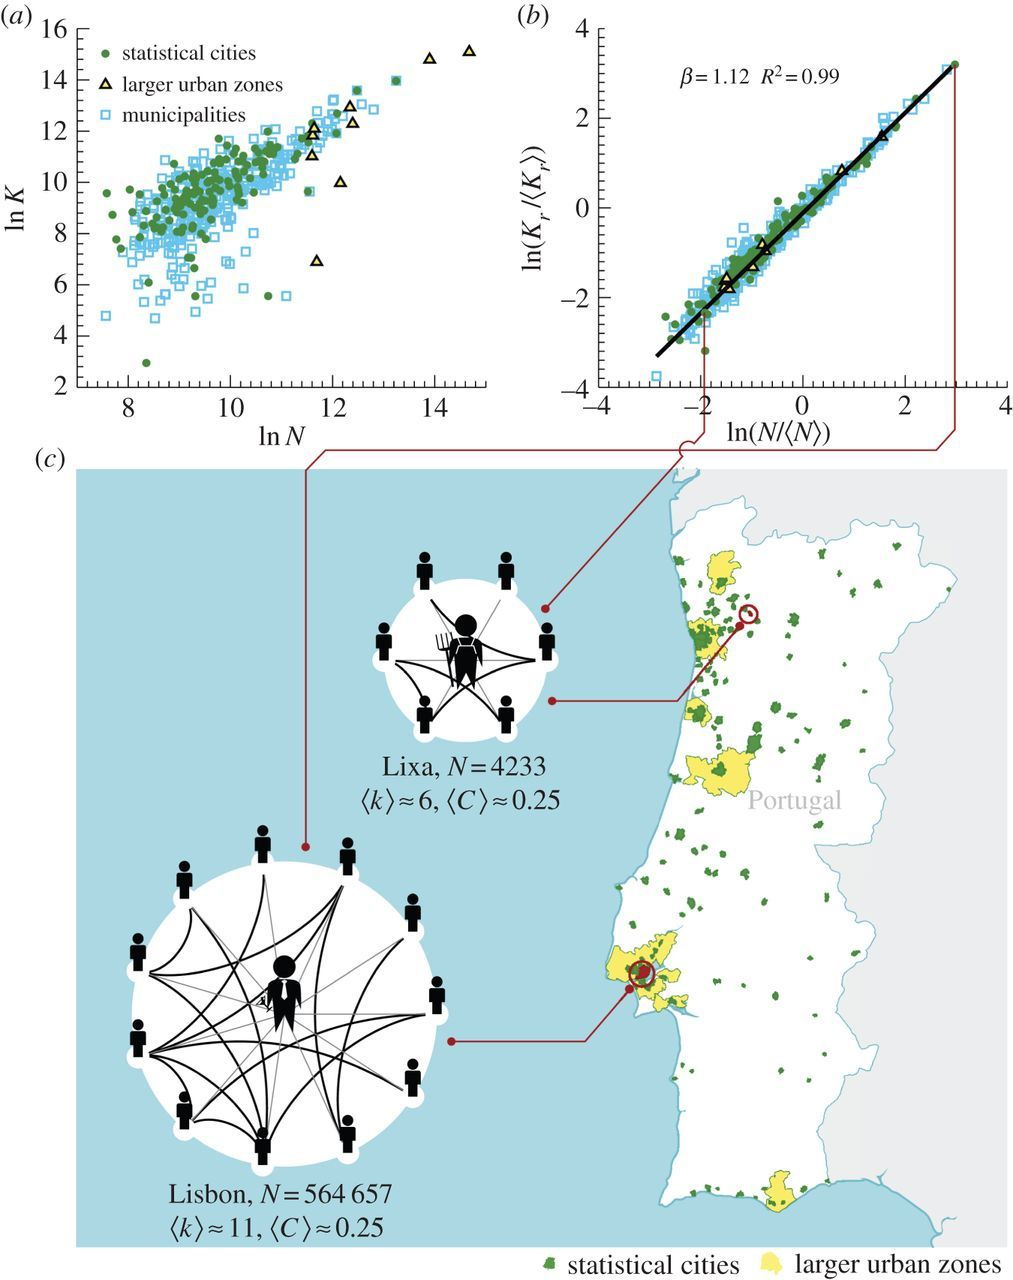
\includegraphics[width = \linewidth]{pictures/rsif20130789f01.jpg}
%     \caption{出自\cite{schlapfer2014scaling},人群交互随着城市规模是一个超线性的关系。}
% \end{figure}

其次是主方程(master equation)。主方程描述的是群体中拥有度为$k$的点所占的比例随时间的变化规律,是一个群体角度衡量城市贫富变化规律的工具。在随机数学中,主方程可以用来描述群落中种群数量的变化规律。由此可见,有一大类问题可以由同样的数理机制解释。我们可以通过对比物理现象中的数量变化过程与经济地理变化规律来扩展更多的结论。对于空间问题,物理中常见的理解方式是通过场论。已经有学者在工作中用到了场论来处理人类移动性在城市内尺度的表现\cite{molas2017field}。该模型提出城市是一个有单中心的实体。这样的实体中人群移动实际上是一个随机梯度下降的过程,即各个空间位置的关系是动态平衡的。在接下来的研究中,我们也会引入随机斩杀模型的Feynman-Kac公式\cite{PhysRevE.98.052114}来进一步解释移动性过程中的交互问题。主方程推导出的场模型另外一个出路,则是利用电场中的性质,结合生态系统理论,来预测城市群的经济关联关系。如果将每个城市考虑为一个电网中的支路,那么\cite{doyle1984random,Volchenkov2011Random}显示,我们可以通过电路分析中的一些算法来求解城市间物质流动的稳态关系。进一步,我们还将在后面根据此算法来讨论更进一步的城市间物质流动的稳态性质。

在空间问题中,异质性是广泛存在的。GN模型中注意到,在研究随机图的矩时,保证低阶矩的稳定的同时增高高阶矩是一个得到网络异速增长的有效办法。这里我可以总结为,空间异质性的形成是由局部升矩过程导致的。我们在研究了其他一类模型之后,发现其他模型得到了同样的构造方式。根据此,我们也提出了自己的新模型来构造这个过程。我们首先在下面一节中介绍几种城市聚集体模型和其中的升矩关系。再在下面一节的后半部分介绍我提出的一种升矩模型。

\section{城市聚集体的模型与偶发事件}

城市形成的物理理论可以分为两个大类:已有人口和资源如何重新聚集继而形成城市;新人口和资源如何增添到已有的城市之中。\cite{PhysRevLett.79.523,PhysRevE.58.295,PhysRevLett.112.240601}提出的模型解释了第一种情况。直接对第二种机制形成城市建模的研究工作比较少。张江\cite{ZhangScaling,LiSimple}的匹配增长模型提供了类似的思路。笔者在近期的一个工作的一部分即是用两条规则来建立城市间人口分布规律。

第一类模型的思想源于数学上的晶格动力学模型。在二维空间格点上每一个格子有相同的初始人口。随着时间的流逝,人口依照某种半随机的方式进行变化,最终停留在我们熟悉的规律上。这种演化方式通常是升矩的。比如Manrubia, Susanna团队在1998年的两篇工作\cite{PhysRevE.58.295, PhysRevLett.79.523}继承了Zeldovich在随机网络的工作,并引领了这个机制在城市科学的相关研究。在人口系统中,地理相关性通常被称为相关场,作为局部人口迁移的动力学机制解释。在总人口为确定值的二维方形格网区域内,记录每一个时刻$t$的每个格点$x$上的人口为$n(x,t)$. 则下一个时刻的人口分布符合\begin{align}
    n(x,t') = \begin{cases}
        (1-q)n(x,t)/p , \text{概率为 } p\notag\\
        qn(x,t)/(1-p) , \text{概率为 } 1-p
    \end{cases}
\end{align}这种机制保证了总人口的恒定,同时(由于均值不等式的成立)增加人口分布的矩$\mu_k(t) = \sum_k n(x,t)^k$。它的实际意义是不断增加的空间异质性。由于总人口的恒定,该模型可以解释为一个人口迁移模型,即人口不断从乡村区域迁移到城市,迁移到不同城市的速率正比于城市的规模。为了使这个机制得以实现,我们还需要假设对于每一个位置,迁出的人口是该处人口数的一个固定比例$\alpha$。
\begin{figure}
    \centering
    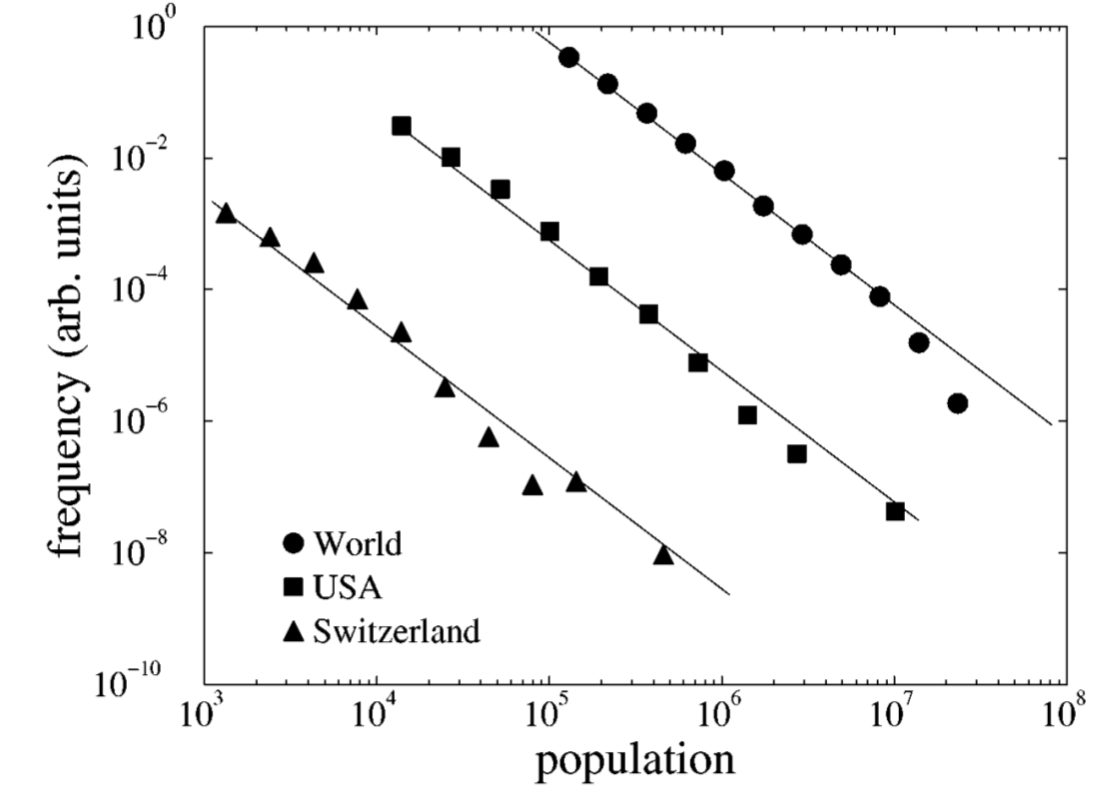
\includegraphics[width = 0.3\linewidth]{pictures/roiiudreal.png}
    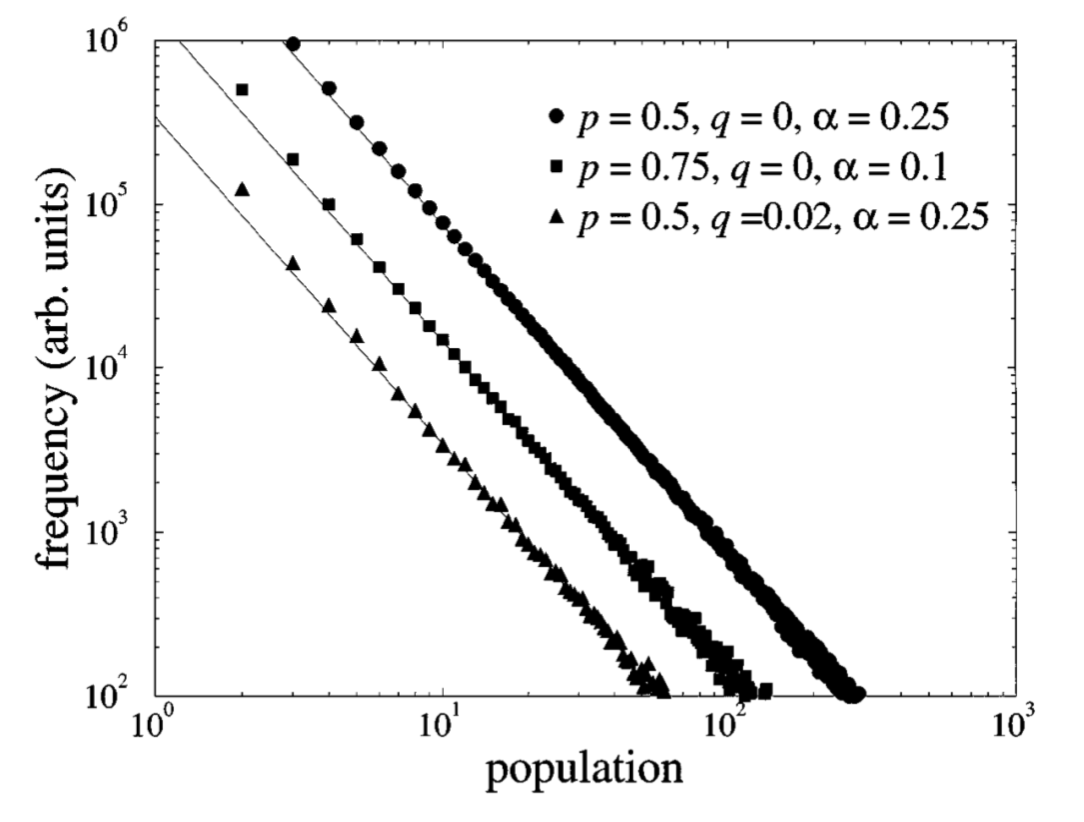
\includegraphics[width = 0.3\linewidth]{pictures/roiiud.png}
    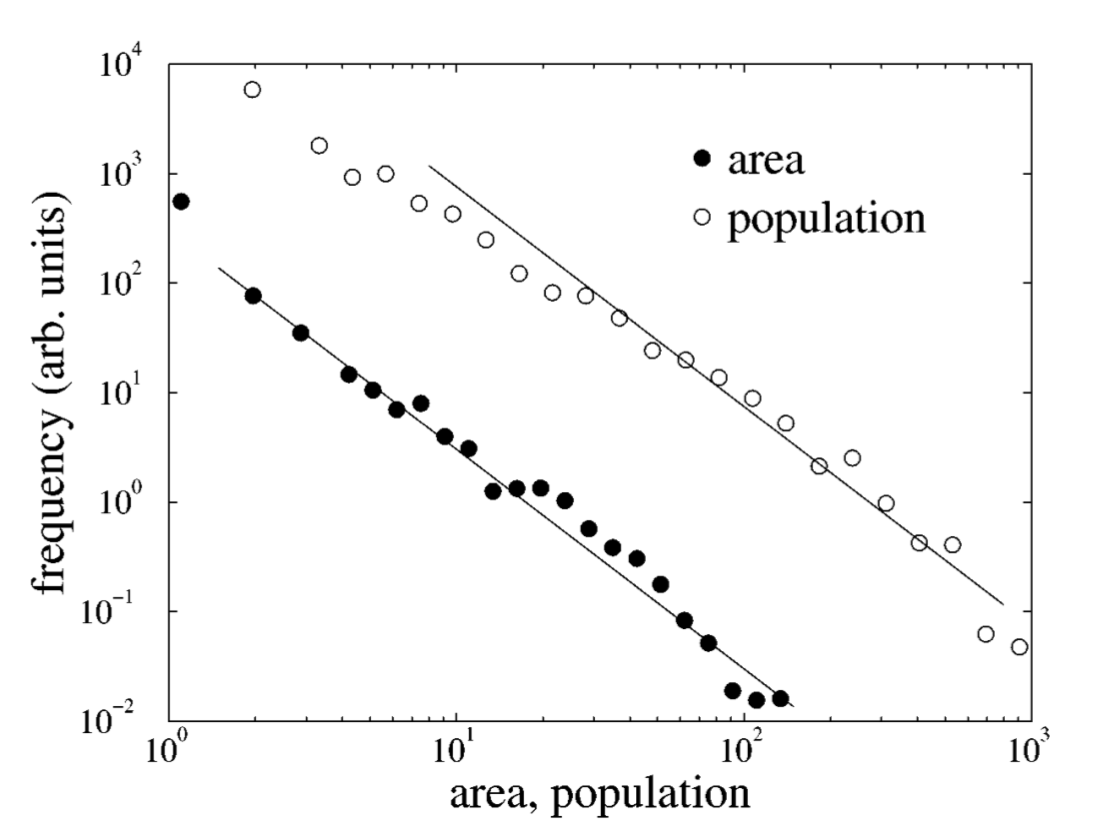
\includegraphics[width = 0.3\linewidth]{pictures/roiiudarea.png}
    \caption{左图:全球2700个最大城市,美国的2400个最大城市和瑞士的1300个最大的自治市的人口分布\cite{PhysRevLett.79.523}。图中斜率为$-2$ 右图是该文中对于不同的参数的三组模拟结果。我们发现,该模型下不同参数导出的城市人口分布都服从一个参数为$2$的幂律分布。}
\end{figure}该模型可以导出的另一个结果是城市面积的频率。通过假设人口密度高于总人口密度的区域为城市区域,连通的城市区域可以进行面积的统计。城市人口的聚集效应导致城市面积趋近于稳定大小。边际区域上面得到的补充人口与扩散人口数维持动态平衡。

Makse,Havlin,Stanley在1995年的文章\cite{Makse1995}中提出的模型进一步解决空间标度律和形态学问题。它符合了两种真实的城市性质。首先,单中心城市的人口密度随着到城市中心的距离是指数衰减的,即\[\rho(r)=\rho_0 e^{-\lambda r}\]其中$\lambda$是密度梯度。其次,在真实的城市中,发展单元在空间上并不是随机分布的,而是以街区的形式规则排列的。并且,发展得好的区域的邻近区域通常也有良好的发展。在地理上,这被解释为空间自相关性。基于这两个假设,作者提出了一个相关渗流模型。一个距离城市中心距离为$r$的景观以概率为$u(r)$被占据。这个概率是基于幂律分布的。该模型生成的城市形态具有明显的分形和随机性特征。模型生成的连通集团可以定义为模型生成的城市边界。大型的城市的吸引力使得郊区城市分中心的边界不及中心城市区紧致(compact)。这与如柏林、巴黎和伦敦等城市的真实情况是相符合的\cite{Batty2006}。笔者的模型中利用了一种新的机制来重现这种性质。即不同城市的扩张是独立的,而大城市在城市边缘的人口密度小于小城市的人口密度。从而在土地竞争中占更劣势,使得小城市的边缘更加突出,从而体现出去紧致化的特征。

该模型其他的性质包括城市面积随着相关距离衰减规律。对于不同的衰减指数,连通面积的频率的衰减规律都是一个指数为$2.09$到$2.45$的幂律分布。
\begin{figure}
    \centering
    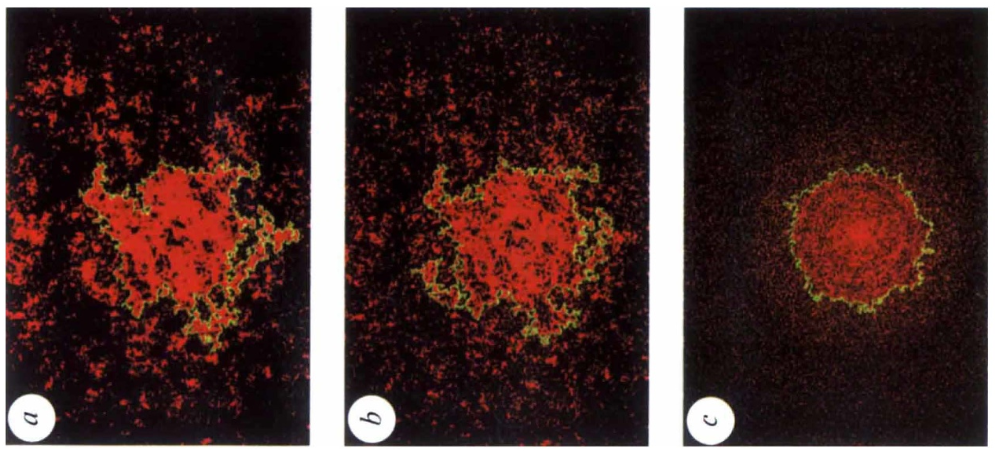
\includegraphics[width = 0.65\textwidth]{pictures/modellingurbanpattern.png}
    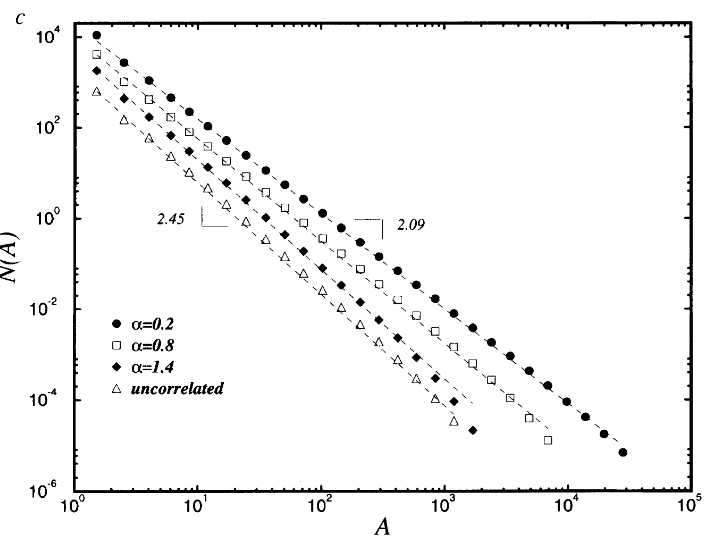
\includegraphics[width = 0.45\textwidth]{pictures/area_scaling.png}
    \caption{上方是\cite{Makse1995}中的模拟结果。前两图分别为幂律指数为$0.6$和$0.4$的情形。可以看出,随着幂律指数的升高,城市的“斑图化”更加明显。城市郊区形成副中心的概率更高。最后一张图表示完全随机的情形,即不同景观之间的发展完全不互相影响。下方是\cite{Makse1995}模型导出的城市面积分布规律。在这里我们认为一个连通的组团是同一个城市。}
\end{figure}

Rybski等人在\cite{PhysRevE.87.042114}中提出的模型是上述观点的扩展。该模型基于的假设是:增长更可能发生在居住空间附近。这个效应由一个距离衰减系数控制。具体实现是每次对所有位置遍历,如果它收到的来自于其他区域的总放射量大于某个阈值,那么这个位置就会被标记为城市区域。这个过程也可以迭代进行。该模型模拟出的城市面积分布与真实情形在统计意义上是相似的,都是幂指数为$2.5$的幂律分布。

值得注意的是,该模型是一个基于距离衰减的长程模型。该模型更显著的特征是对于位置间的关联通过距离加权,进而得到局部的发展潜力。我们认为这种模型是与重力模型有很大关系。尽管人口引力一词在国民经济学领域是Stewart于\cite{10.2307/2785468}提出的,但在经济地理研究中,引力模型已经研究了数十年。 Carrothers\cite{carrothers1956historical}对重力和人类互动的潜在关系进行了综述。销售行业的瑞利引力定律描述了相同吸引力的边界范围\cite{reilly1931law},它依赖着销售业和城市居民的同质性假设。Huff的购物者吸引力定律\cite{10.2307/3144521}提供了代理商在给定地点前往特定设施的可能性。重力模型则可以用来做国家之间的贸易量的建模。它的局限性是在流动和迁移问题建模时,无法反映非对称的情形。有工作将重力模型修正为\[G_{ij} = \frac{m_i^am_j^b}{d_{ij}^c}\]用以回应不对称的情形,但该模型需拟合的参数过多,降低了模型的解释性。可见重力模型在地学和经济学问题中扮演了举足轻重的地位。空间占领背景下的重力模型是比较容易被忽略的,因为被占领的空间的质量只是$1$,从而没有重力模型下强异质性场的问题。\cite{PhysRevE.87.042114}中的模型建立在$N\times N$栅格空间上每两个栅格之间的作用强度由下式定义:\[q_j = C\frac{\sum_{k\ne j}w_k d_{ij}^{-\gamma}}{d_{ij}^{-\gamma}}\]可以看出这个模型的权重项跟Huff模型的吸引力是一样的,并且其中的衰减系数$\gamma$的增大会使得距离衰减更快,进而增加模型的集聚效应。每一个时刻,每个栅格都会评估一下其余栅格对其的总作用。如此迭代下去,会形成一些染色图案。\begin{figure}
    \centering
    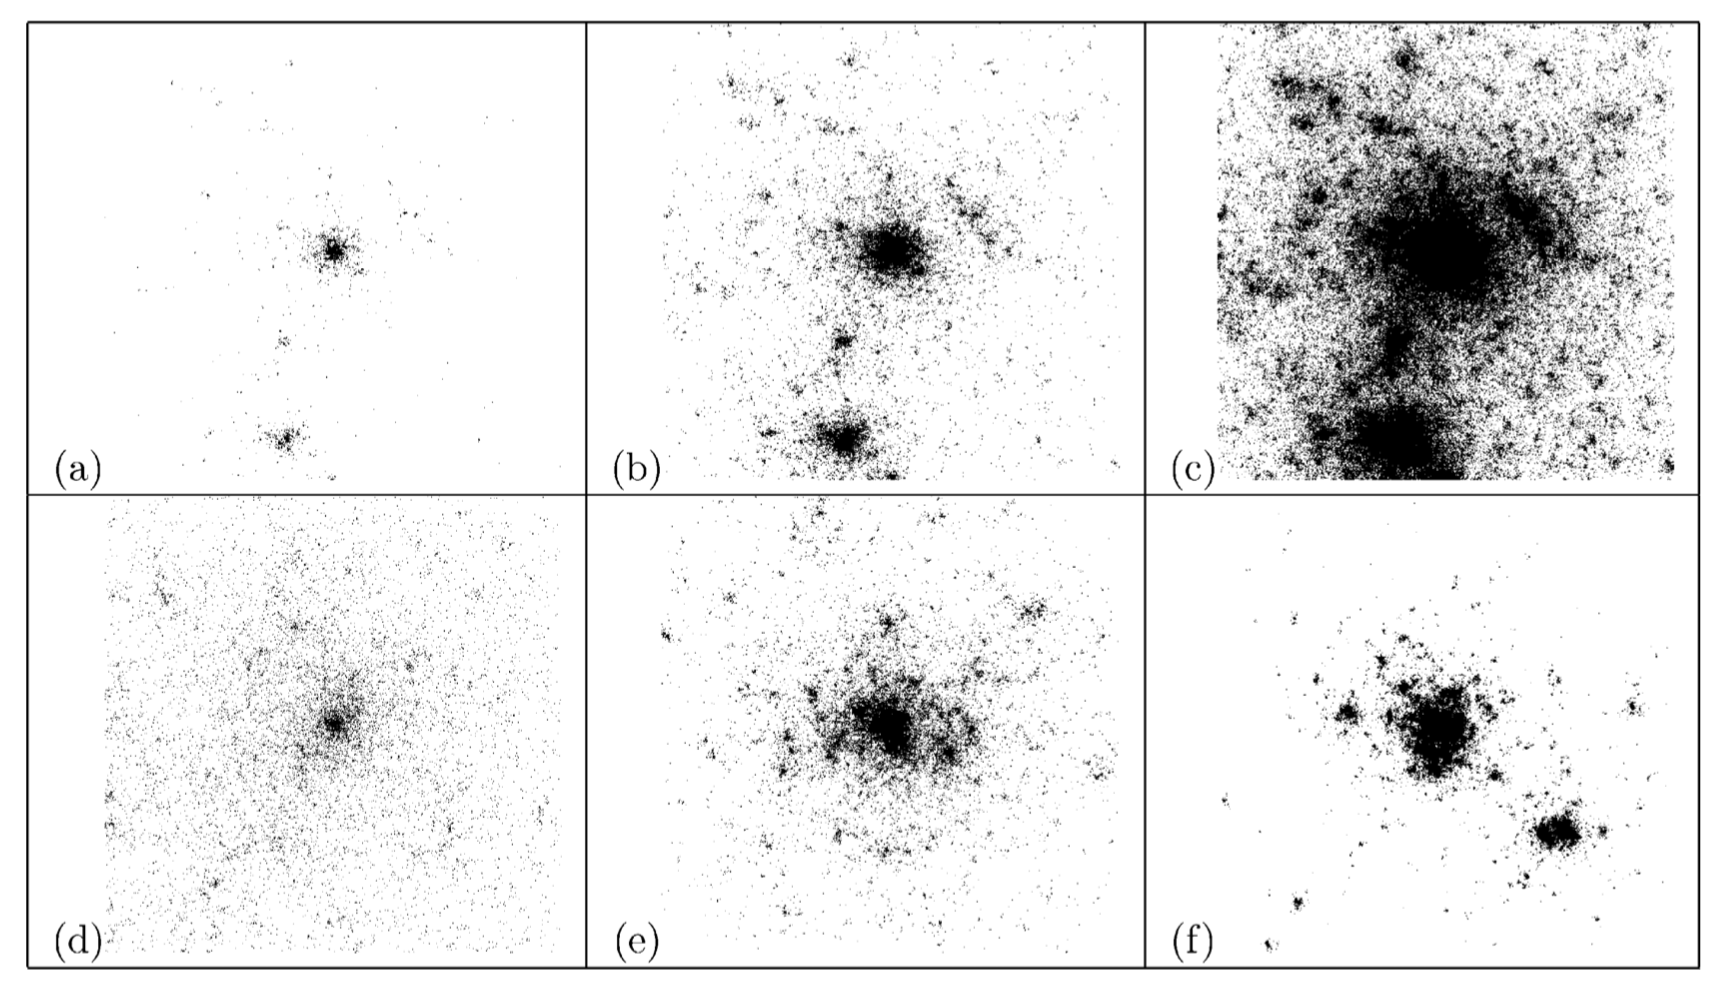
\includegraphics[width=\textwidth]{pictures/distance-weighted.png}
    \caption{前三个图是模型迭代6,10,14次的图案;后三个图是距离衰减指数为2.0,2.5,3.0时的城市分布。}
\end{figure}
该模型导出的统计结果可以概括为三条:城市面积的幂律分布、城市边界的分形、以及区域连通性的渗流相变。

基于此类模型,笔者总结了较为一般的模型规律。即反应-扩散模型(reaction-diffusion models)导出空间异质性的基本原理。这一模型假设在城市形成的过程中地理位置上相邻的区域具有高的交互强度(reaction),而相邻区域的人口分布差异促进了人口流动(diffusion),差异越大,人口分布的变化趋势越明显。动力学的升矩过程描述了差异增大的过程,可作为空间异质性增强的合理假设。在$N\times N$的二维格点空间中,给定各个格子分布1单位人口为初始状态。模拟城市生成的迭代规则基于反应与扩散机制——在内部($N-2$)$\times$($N-2$)的格点中以某一指定的顺序遍历格点,通过比较目标格点与其八邻域人口均值($n_{neighbor}$)的相对大小更新格点人口数目,模拟人口迁入($\geq n_{neighbor}$)或迁出(\textless$n_{neighbor}$)过程。具体来讲,假设人口迁出比例为固定的$\alpha$,则目标区域的更新规则为:

\begin{equation}
n(x,t) 
\begin{cases}
	<\overline{n(\delta x,t)}: & n(x,t)=(1-\alpha)n(x,t) \notag\\
	 & n(\delta x,t) += \frac{\alpha}{8}n(x,t)\notag\\
	\geq\overline{n(\delta x,t)}: & no\ change
\end{cases}
\end{equation}
其中,$x$为目标格点,$\delta x$为其八邻域,$\overline{n(\delta x,t)}$为八邻域格点内的人口均值。人口数越多,区域的吸引力越强,就会有更多的人口迁入。在此模型中,更新只在目标格点人口低于邻域均值时进行。我们不考虑人口数值外的其它区域环境差异因素,因此低值格点会均匀地向其八邻域迁出$\frac{\alpha}{8}$比例的现有人口。

这一基于反应-扩散机制的城市生成模型,根据人口分布特征与基本的交互规则模拟城市生成过程,由均匀到聚集分布的升矩机制可以从动力学角度对空间异质性的产生原理进行解释。由此可进一步探讨城市区域性差异及形态学问题:目标格网的选取顺序对人口更新过程及城市格局形成的影响,如随机选取,横向遍历,由中心向四周遍历等;模拟的人口频数分布与Clark定律的吻合程度可对模型进行验证;通过格点人口数阈值(如格点数值小于1)可提取城市范围及平均半径,进而对城市面积量化与形态学研究提供参考。

% 还有Potts models

\section{考虑人口密度的空间生长模型}

我们可以看出传统的格点网络框架将城市发展的范围作为最重点的研究对象,这对传统的城市扩散有着比较好的效果。但是随着城市的发展,越来越多的城市都会集中在相对固定的区域上。在每个城市内部,高楼的数量会越来越多,更多的城市资源会向城市中心集中\cite{BerryThe}。这时,我们再用格点模型和斑图动力学来研究空间问题将不够恰当,因为这些模型只能研究空间问题的一些很片面的方面。我们需要考虑空间上小地块上的密度,所以基于连续空间上的点过程就变得尤为重要。

我们先考察匹配增长模型\cite{zhang2015scaling}。该模型的过程是这样的:给定一个有界\(d\)维欧式空间\(S=|x_1|,\cdots,|x_d|\leq \frac{L}{2}.\) \(t=0\)时在原点插入一个结点。结点生成的机制为:每个时刻\(t\),以均匀分布在\(S\)中放置一个新结点\(P_t\),记它的坐标为\(x_t.\) 如果存在一个已有结点\(P_q,q\in\{1,2,\cdots,t-1\}\),跟这个新生成的结点很接近,使得\(||x_p-x_q||< r\),则新结点\(P_t\)存活,否则\(P_t\)死亡。连边机制为:将新加入结点与其\(r-\)临域的所有结点相连。重复这个过程,直到存活的结点达到\(N\)个。因为新加入的结点可生存的区域的测度(为所有存活结点的\(r-\)临域的开覆盖)会越来越大,这个几何网络会加速增长。
\begin{figure}
    \centering
    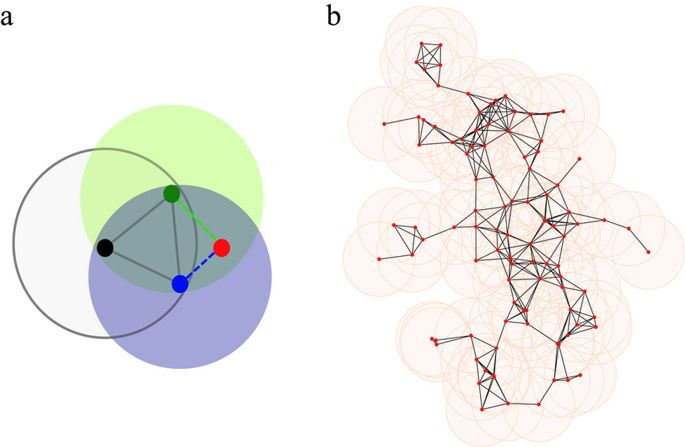
\includegraphics[width = 0.48\textwidth]{pictures/srep09767-f1.jpg}
    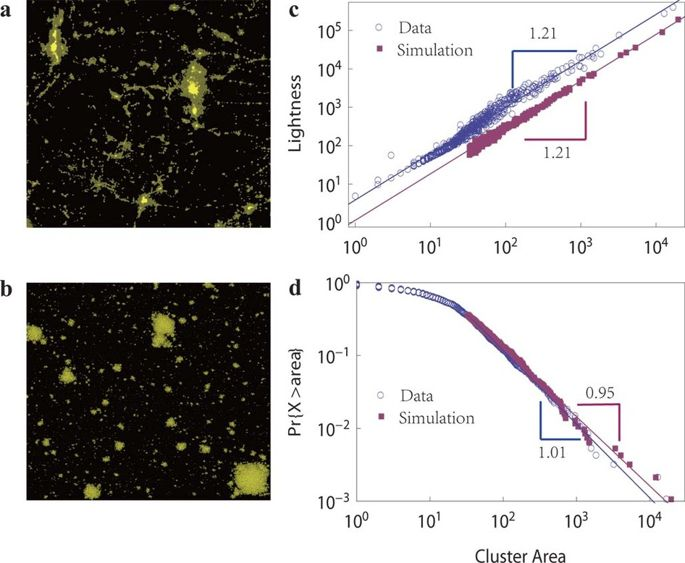
\includegraphics[width = 0.48\textwidth]{pictures/srep09767-f3.jpg}
\end{figure}

这个模型在一定程度上是可以解析的。由于模型的各项同性,在取热力学极限($L,t\rightarrow\infty$)的情况下,这个空间网络会渐近形成一个$d$维球。于是模型给出的第一个性质,也就是这种机制下网络空间的半径$R(t)$是正比于时间的。半径\(R(t)\)(定义为\(\max\{||P_0-P_i||,i=1,2,\cdots t\}\))。以1维正半轴为例,新结点\(P(t+1)\)落在\([0,R(t)+r)\)可以生存,落在\([R(t)-r,R(t)+r]\)可以使得\(R(t+1)> R(t).\)于是增加半径的量的期望为(在\(R(t)\)远大于\(r\)的前提下)
\begin{align}
  &\int_0^Ldx\ P(x_{t+1}=x)\Delta R_{x,t}\notag\\
  =& \frac{2r}{L/2}\int_{R(t)-r}^{R(t)+r} dx\ \frac{1}{2r} (x+r-R(t))\notag\\
  =& \frac{2}{L} \{(2r\cdot [r-R(t)]) +\frac{1}{2}[(R(t)+r)^2-(R(t-r))^2] \}\notag\\
  =& \frac{2}{L} 2r^2\notag\\
  =&r^2/L\notag\\\
  \equiv& C 
\end{align}
所以网络的半径\(R(t)\)匀速增长。所以\(R(t)\sim t\)。对于多维情形,在每个维度上的半径\(R_1,\ldots,R_d\)的增长速率都相同,所以它们的线性组合的增长速率相同,即向任何一个方向的增长速率相同。

第二个问题则是点密度问题。距中心距离为\(\rho\)时,密度\(\mu(\rho,\Theta ,t)\sim \frac{R(t)-\rho}{L^d}\),\(\mu(\rho,t) \sim \frac{(R(t)-\rho)\rho^{d-1}}{L^d}. \)到中心距离在\(\rho\)以内的结点个数\(\sim \rho^d\)。利用这个关系,我们还可以得到存活下来的结点总数以及边数。总人口为:\begin{align}
    N(t)&=\int_0^{R(t)}\mu(\rho,t)d\rho\notag\\
    &\sim R(t)^{d-1}\notag\\
    &\sim t^{d-1}
    \end{align}边数为边数\(v(\rho,\Theta,t)\sim u(\rho,\Theta,t)^2\)(局部每两个边都相连),所以总边数可以写为\begin{align}
        E(t) &=\int v(\rho,\Theta,t)d\sigma\notag\\
&\sim \int t^2\cdot t^{d-1} dt(\text{极坐标变换})\notag\\
& =t^{d+1}.
    \end{align}所以我们有$E(t)\sim N(t)^{\frac{d+2}{d+1}}$。这个结果与\cite{PhysRevX.4.011008}的结果是类似的。这说明局部全连接形成的变化趋势与空间社交网络形成的长短程交替建立的连接强度是类似的。

    该模型可以通过增加一个参数得到更符合真实世界结果的解析解。事实上,真实世界中一个人来到某个城市,如果举目无亲,他也有一定的正概率扎根下来。
    一个新加入的结点的生存概率是插入点的点密度的一个负指数倍:\[P(\text{survive})=\mu(\rho,\Theta,t)^{-\alpha}\]与之前的推导类似,在某位置\(d\sigma\)附近的结点个数为\[\mu(\rho,\Theta,t)d\sigma = \int_{\tau_\rho}^t \mu(\rho,\Theta,s)^{-\alpha} \frac{d\sigma}{L^d}ds\]我们可以得到一个偏微分方程:$
        \frac{\partial u}{\partial t} =\frac{1}{L^d}\mu^{-\alpha}$,并以$\mu(\rho,\Theta,\tau_\rho)=0$为初值条件。它的解是\[\mu(\rho,\Theta,t)\sim(t-\tau_\rho)^{1/(1+\alpha)}\]这使得我们得到了边和城市体积的修正分布规律:边:\(R(t)\sim N(t)^{1+\frac{1}{1+(1+\alpha)d}}\),体积\(V(t)\sim N(t)^{1+\frac{1+\alpha}{1+(1+\alpha)d}}\)。当\(\alpha\rightarrow\infty\)时,上述两个幂律指数都会趋近于\(1\)。也就是随着\(\alpha\)的增加,超/亚线性性会降低至线性。

这个工作有一些潜力在空间上得到几何相-无标度相的相变\cite{balister2018topological,rozenfeld2010small}。我认为两种相的本质区别在于是否个体大小可以忽略。如果可以忽略,则体现出更集体性、层次性的无标度相;反之则是几何相,或者成为小世界相。

\section{生长模型的记忆效应、城市的兴衰变迁}

城市的发展是历史累积的,是在高度异质性和差异性的环境中不断演化的。而生长模型中,如果将大多数机制建立在无记忆性的指数增长过程中,模型对于复杂历史状况的城市演化规律的解释能力就会有所下降。生长模型本身的研究过程也在不断引入新的改进机制,从而使得模型仍能预测出较为确定的指标(可解析性,以及更多的考察要素,如Taylor定律\cite{Giometto7755}),也能得到更符合实际状况的预测效果。事实上生长模型中加入有限的记忆效应是很多工作考虑改进的方向\cite{Schaigorodsky2018}。一方面随着时间增加,虽然生长模型不会爆炸,但是后期性质显示真实情形中,我们完全不可以忽略人的大小,即抑制进一步发展的拥挤是真实存在的。另一方面年龄结构也是社会主流问题。生长模型作为一种纯生的机制,并不完全适合存在演替的城市生态系统。

Durrett在\cite{gleeson2017temporal}中探讨了在雪崩形成过程中,历史积累的情况。一个事件引起一个或多个后续事件时,就会发生雪崩或级联,进而可能导致连锁反应中的其他事件。在许多学科中研究雪崩动力学,最近集中在平均雪崩形状上,即固定持续时间的雪崩的时间分布。在动力学角度,不同持续时间的重整化后的平均雪崩形状会退化到一条通用曲线上。我们应用马尔可夫分支过程理论来推导控制网络级联动力学的平均雪崩形状的方程。临界状态下的方程分析表明,对于某些动力学和网络拓扑组合,会出现非对称平均雪崩形状(在某些实验中观察到)。该模型的数值模拟可以给出对于信息传播,神经动力学和行为接纳这几个不同领域都适用的解释,并提出简单的实验测试来量化级联系统是否处于临界状态。该文章的思想说明,我们可能处于某个分形状态的某个分支中,我们知道世界是自相似的,但是我们并不知道这个高度随机的系统有多少是可以被观测的。即我们很难知道分型的维数。所以建立与观测对应得最好的一种生成模型始终是有意义的。虽然这个模型可能高度不确定,但是我们仍然可以通过多次模拟预测可能的轨迹。这是生成模型中,历史的重要性。

Jackson在\cite{akbarpour2018diffusion}中表示,疾病的蔓延和信息的传播取决于个人的接触。人们并不总是能够与周围的人互动,并且人们活动的时机决定了人们是否有机会会面和传播细菌、想法等,并最终决定是否会广泛传播或传播。简单地来讲,邻居不一定都会互相认识,尤其是我们这个社交环境严重拓扑化的时代。文中证明,在一个简单的传染或扩散模型中,当活动模式存在异质性时,最大程度的传播发生:有些人长时间处于活动状态,然后长时间不活动,仅偶尔改变其可用性,而其他人经常在活跃和不活跃之间交替。这个事实对限制传染性疾病以及促进信息传播具有政策意义。这也显示了我们对一个人行为模式的理解有助于预测它在社会网络中的影响力。

Gleeson的研究\cite{gleeson2016effects}表明,在线社交媒体极大地影响了我们彼此交流的方式。但是,人们对什么基本机制驱动在线社交系统中的动态信息流知之甚少。文章中提出了一种在线共享行为的生成模型,该模型在分析上易于处理,并且可以复现有关标签使用情况的经验微博数据的多个特征,例如(时间相关的)模因子流行度的重尾分布。 所提出的框架构成了社交传播现象的空模型,与纯粹的经验研究或基于模拟的模型相比,该模型清楚地区分了影响模因流行的两个不同因素的作用:用户的记忆时间和社交网络的连通性结构 。

Batty在nature文章\cite{Batty2006}中引入了一种新的概念:序时钟。研究显示,在美国建国的210年间,有266个城市在某个阶段进入了前一百名;1840年城市数量首次达到一百,这一百个城市只有21个在2000年仍然是前一百的城市。平均而言,一百个城市里,一半的城市出现或消失所需在前百表单的时间为105年,而城市的平均排名变化速率是每十年为七个位次。所以可见城市的兴衰变迁是常见且有规律的。这很容易理解:不同的时代有着不同的价值观。不同时代的国家也有着不同的支柱产业和经济重心,所以每个城市会有属于自己相对优势的一段时期。

\begin{figure}
    \centering
    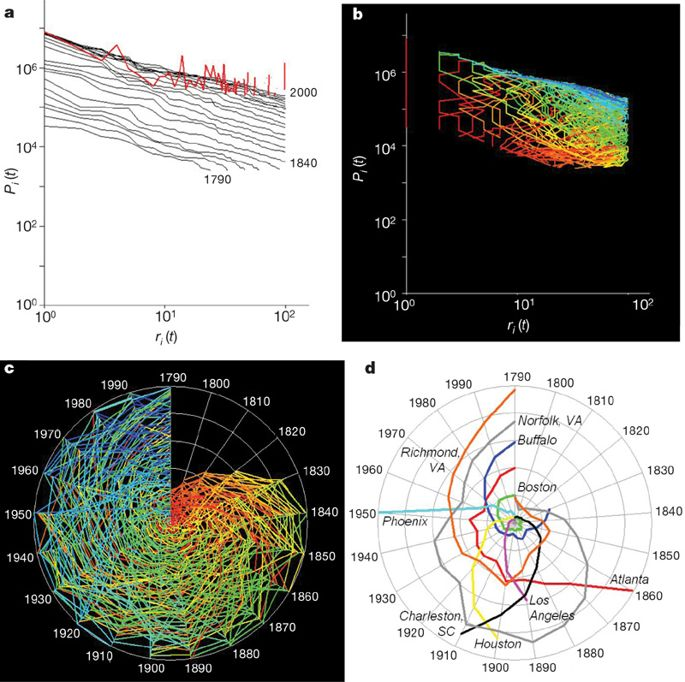
\includegraphics[width = 0.9\linewidth]{pictures/rankclocks.jpg}
    \caption{出自\cite{Batty2006}。图(a)是每个Zipf图。每条线代表一年的城市排名与城市规模的关系。红色线是1950年的城市排名与2000年的人口构成的点对练成的线。(b)是不同城市位序随时间的变化规律。(c)则是序时钟。每个点到圆心的距离代表它的排名。(d)图是几个城市的序时钟轨迹。}
\end{figure}

我提出了一种解释城市兴衰演变的机制。并在我之前提及的生成模型中加以使用,得到了很好的结果。该模型进而解释了城市多中心的出现以及城市收缩\cite{martinezfernandez2012shrinking}现象的出现。在已知的统计物理模型中,城市系统在空间限制和经济投入限制下的动态演化机制还是一个较少被理解的话题。本文中借鉴了空间网络中的匹配增长模型的思想方法和随机过程中的尤尔西蒙模型框架,提出了空间尤尔模型(spatial Yule model,SYM),来考虑城市的生成机制,以期达到在有足够随机性的前提下得到城市的空间分布的一般模式。

我们考虑逐渐一个逐渐出现新城市的方形空间。与此同时,人口也逐渐地加入这个城市系统中。但是只可以加入已经存在的城市中。由于城市的加速生长属性,每个城市中的新人,都是一个已经在这个城市定居的人带来的,所以它们定居的位置会在已经定居的人的一个邻域范围内。为了建模的方便,我们认为,这个位置就是前人定居位置的一个随机方向上的一个固定步长所确定的位置。接下来我们要描述占领机制。由于有自上而下生成城市的假设存在,以及行政区划的限制,我们认为一个城市的人口在占领了一个区域之后,这个区域的归属权就不会易主了。而在模型之前的假设中,每个人又只是一个质点。我们需要给他一个可以控制的最小区划单元,来作为占有机制,排除其他城市的侵占。所以我们将空间分为$N\times N$个小方格,也即将空间打上横N纵N的线。这种操作也相当于假设每个格子的长宽都规定为1。每个格子归属于哪个城市,取决于落在其上面的第一个人口的户籍所在。在此之后,如果新的同城市结点落在这个格子上,那么它就可以生存下去;而其他城市的结点落在这个城市的区域上的时候,则会立即死亡。也就是说,我们给了这个模型的区域占领完全的先入优势。这也是经济学中常见的假设。

最后的一个假设是模型的关键。对于一个区域的建设来说,通常有一个建设的瓶颈,即来自上层的经济投入。比如说,对于中国来说,近些年来的经济增长上限一直是比较固定的。在全球经济环境的限制下,我国的GDP年增幅一直在$7\%$左右。也就是说,我们在每时每刻创造的财富的价值是有其上限的,并不能随着时间单调递增。而在本模型的考虑中,每个新的人口加入城市所需要的培养成本可以认为是相同的。于是我们增加一个“记忆核”的限制,使得只有有限个结点可以产生子结点。即每个人加入我们考虑的空间的时候,要先在这个记忆核中“登记”,再加入这个空间。而这个记忆核的大小是有限的,我们记它的大小是$N^*$,那么如果记忆核已经被填满了,新结点的加入,就会挤出一个旧结点。这样就相当于对系统的生长增加了一个经济指标的限制,从而使其更贴近现实。

该模型可以解析地导出区域内城市规模地Zipf分布;单中心城市人口密度的Clark分布;以及城市边缘的分形行为。但是我们不满足于此。记忆核机制相当于制作了$N^*$枚金币。在城市人口很少的时候,每个来城市淘金的人都能分到一枚金币。他们也可以用这枚金币在城市的某个地点买一层房子。随着时间的流逝金矿逐渐被耗尽,新加入的人就只能从已有的人的手中拿金币来在城市某处安家。我们以空间为研究对象的话,金币的空间分布可以理解为社会财富的分布。在开始阶段,大家都围绕着城市中心转。在后期资源开始不够了,边缘地区的金币由于密度低,就更容易消失殆尽,进而导致城市收缩。当然,这个过程也有着一定的随机性,导致旧中心转移到了新的中心,或者旧中心保留的同时,城市出现了新的中心。总之,在这个模型中,城市多中心现象和城市收缩现象都是由于有限的社会资源在空间上的配置问题。